\documentclass{article}
\usepackage[utf8]{inputenc}
\usepackage[T1]{fontenc}
\usepackage[polish]{babel}
\usepackage{graphicx}
\usepackage{hyperref}

\title{FM Terapia Antyprotonowa w Leczeniu Nowotworów}
\author{Leon Wojtachnia, Jakub Wołejko, Ignacy Rugowski, Tymon Szymański}
\date{May 2026}

\begin{document}

\maketitle

\section{Cel projektu}
Głównym celem projektu jest teoretyczna i numeryczna analiza możliwości zastosowania wiązek antyprotonowych w radioterapii onkologicznej, jako innowacyjnej metody leczenia nowotworów. Terapia ta ma na celu stanowić odpowiedź na dotychczasowe ograniczenia fizyczne oraz biologiczne metod napromieniania. Ma oferować precyzyjność w niszczeniu chorych tkanek przy jednoczesnym omijaniu zdrowych narządów pacjenta.

\section{Opis problemu}
Głównym problemem współczesnej onkologii jest biologiczna oporność niektórych typów nowotworów na klasyczne metody radioterapii. Wynika to przede wszystkim ze zjawiska hipoksji, czyli stanu, w którym tkanki organizmu otrzymują zbyt małą ilość tlenu w stosunku do ich zapotrzebowania, co występuje głównie we wnątrzu dużych guzów. W takich przypadkach standardowe promieniowanie rzadkojonizujące jest mało skuteczne, a jego skuteczność spada nawet dwu- lub trzykrotnie. Dzieje się to dlatego, że fotony nie niszczą komórek bezpośrednio: jonizują wodę w komórkach, tworząc wolne rodniki, które uszkadzają obie nici DNA. Kolejnym problemem fotonów jest brak piku Bragga, co oznacza, że fotony oddają swoją energię na całej długości przenikania przez ciało i narażają zdrowe tkanki na niepotrzebne i szkodliwe promieniowanie.

Aby skutecznie ominąć tę barierę niedotlenienia i zneutralizować komórki hipoksyjne, współczesna fizyka medyczna musi zastosować promieniowanie o wysokim liniowym przekazie energii (LET). Promieniowanie to nie wymaga obecności tlenu, ponieważ jego gęstość jonizacji jest wystarczająco duża, aby wywołać bezpośrednie i nieodwracalne uszkodzenia struktury DNA (tzw. \textit{Double-Strand Breaks}, DSB). Rozwiązaniem tego problemu jest właśnie terapia antyprotonowa. Łączy ona w sobie precyzję przestrzenną z ogromnym, lokalnym oraz gęstym jonizowaniem jądrowym. Pozwala to na zatrzymanie cząstki dokładnie na poziomie guza, gdzie dochodzi do jej zniszczenia, unikając przy tym tkanek występujących przed i za guzem, dzięki czemu są one bezpieczne.

\section{Fizyka oddziaływania antyprotonów z materią}
Założeniem terapii antyprotonowej jest skierowanie wiązki cząstek o ściśle określonej energii początkowej na nowotwór. Przechodząc przez tkanki, antyprotony oddziałują z nimi, tracąc przez to swoją energię kinetyczną. W celu uproszczenia naszego modelu przyjmujemy, że tkanka miękka wykazuje właściwości zbliżone do wody. Zdolność hamowania opisuje tu równanie Bethego-Blocha:
\begin{equation}
    -\frac{\mathrm{d}E}{\mathrm{d}x} = \frac{4\pi N_{\mathrm{A}} Z \rho}{A m_{\mathrm{u}} m_{\mathrm{e}} c^2} \left( \frac{e^2}{4\pi\varepsilon_0} \right)^2 \frac{z^2}{\beta^2} \left[ \frac{1}{2} \ln \left( \frac{2m_{\mathrm{e}} c^2 \beta^2 T_{\mathrm{max}}}{(1 - \beta^2) I^2} \right) - \beta^2 - \frac{\delta}{2} \right]
\end{equation}

Gdzie poszczególne symbole oznaczają:
    $N_{\mathrm{A}}$ -- liczba Avogadra, 
    $Z$ -- liczba atomowa ośrodka (tkanki),
    $\rho$ -- gęstość ośrodka,
    $A$ -- liczba masowa ośrodka,
    $m_{\mathrm{u}}$ -- stała masy atomowej,
    $m_{\mathrm{e}}$ -- masa spoczynkowa elektronu,
    $z$ -- ładunek cząstki padającej (dla antyprotonu $z=-1$),
    $\beta$ -- prędkość cząstki wyrażona w ułamkach prędkości światła ($v/c$),
    $T_{\mathrm{max}}$ -- maksymalna energia kinetyczna, jaka może zostać przekazana elektronowi w pojedynczym zderzeniu,
    $I$ -- średni potencjał jonizacyjny atomów ośrodka,
    $\delta$ -- poprawka uwzględniająca efekt gęstościowy (polaryzację ośrodka). 
    Pominięto wyjaśnienie stałych powszechnie rozpoznawalnych.


\begin{figure}[htp!]
    \centering
    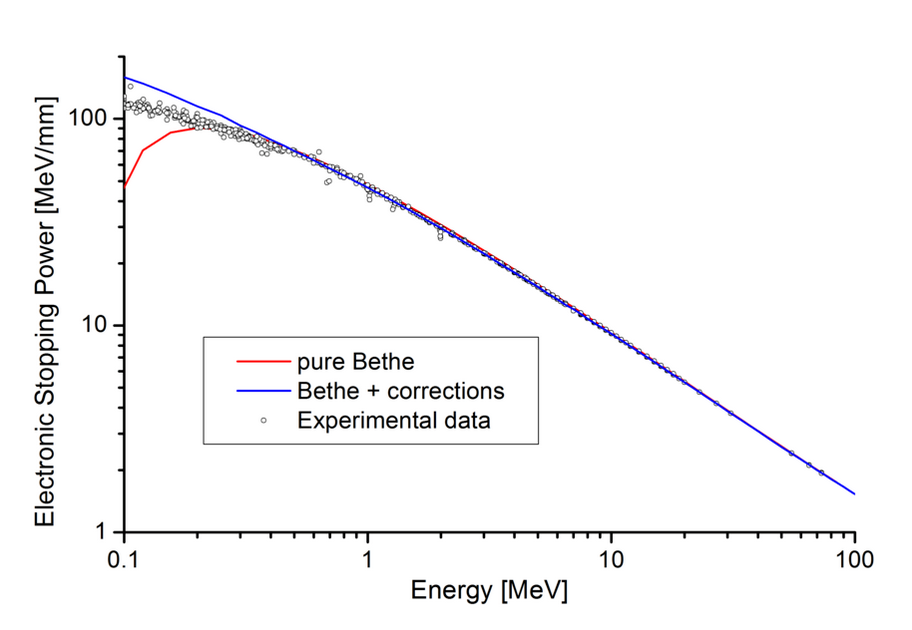
\includegraphics[width=0.75\linewidth]{obraz.png}
    \caption{Ilustracja piku Bragga (źródło: Wikipedia)}
    \label{fig:bragg_peak}
\end{figure}

Zgodnie z charakterystyką oddziaływania tej cząstki, utrata energii jest odwrotnie proporcjonalna do kwadratu jej prędkości. Prowadzi to do intensywnego wyładowania pozostałej energii pod koniec lotu, co określa się pikiem Bragga. Symulację numeryczną ilustrującą utratę energii antyprotonu w funkcji głębokości penetracji, na której wyraźnie widoczny jest ten pik, udostępniliśmy w repozytorium projektu: 

\url{https://github.com/Le-ON-Crazol/FM-Terapia-Antyprotonowa-w-Leczeniu-Nowotwor-w/tree/main}.

Główna różnica pomiędzy klasyczną radioterapią protonową a antyprotonową jest widoczna w momencie zatrzymania cząstki. Po utracie energii kinetycznej antyproton zostaje przechwycony przez jądro pobliskiego atomu tkanki, gdzie łączy się z jednym nukleonem i ulega natychmiastowej anihilacji, w wyniku której uwalniana jest energia spoczynkowa ok. $1{,}88~\mathrm{GeV}$. Prowadzi to do rozpadu jądra atomowego i emisji wysokoenergetycznych fragmentów (np. cząstek $\alpha$, powolnych protonów oraz jąder odrzutu), co określa się gwiazdą anihilacyjną. Emitowane cząstki mają bardzo krótki zasięg (rzędu milimetrów), co pozwala na precyzyjne ograniczenie działania tylko do obszaru guza, minimalizując szanse na uszkodzenie zdrowej tkanki.

Do obliczeń wykorzystuje się przybliżenie ciągłego spowolnienia (CSDA), które pozwala na całkowanie utraty energii wzdłuż całego toru lotu. W celu optymalizacji tych obliczeń wykorzystuje się prawo skalowania zasięgu oraz reguły potęgowe (np. reguła Bragga-Kleemana).

\section{Alternatywne cząstki}

W celu pełnego zrozumienia zalet terapii antyprotonowej, przeprowadzono numeryczną analizę porównawczą dla innych rodzajów promieniowania uwzględnionych w symulacji. Zbadano następujące cząstki:


\subsection{Jony węgla ($^{12}$C)}
\textbf{Zalety:} Charakteryzują się niezwykle ostrym pikiem Bragga oraz wysokim współczynnikiem LET. Doskonale radzą sobie z komórkami hipoksyjnymi, trwale uszkadzając ich DNA niezależnie od obecności tlenu. \
\newline
\textbf{Wady:} Za pikiem Bragga generują tzw. ogon fragmentacji (lżejsze jony powstałe z rozpadu węgla, naświetlające tkanki za nowotworem). Ich zastosowanie wymaga budowy potężnych i bardzo kosztownych akceleratorów.

\subsection{Elektrony ($e^-$)}
\textbf{Zalety:} Wytracają energię szybko i wnikają bardzo płytko, co czyni je użytecznymi i bezpiecznymi w radioterapii zmian powierzchniowych (np. nowotworów skóry). \
\newline
\textbf{Wady:} Nie posiadają piku Bragga, a ze względu na małą masę silnie się rozpraszają. Dawka opada powoli wraz z głębokością, co całkowicie uniemożliwia ich zastosowanie w leczeniu głęboko osadzonych guzów.

\subsection{Pozytony ($e^+$)}
\textbf{Zalety:} Podobnie jak elektrony, deponują główną dawkę na niewielkich głębokościach, oszczędzając głębsze narządy. \
\newline
\textbf{Wady:} Choć na końcu ich toru lotu dochodzi do zjawiska anihilacji (z elektronami ośrodka), uwalniane są w niej wyłącznie dwa przenikliwe fotony o energii $511~\mathrm{keV}$. Energia ta nie niszczy komórek guza (zbyt niski LET i duży zasięg fotonów), lecz opuszcza pacjenta, niepotrzebnie powiększając tło promieniowania wtórnego.

\section{Metodologia badawcza i obliczeniowa}
Analiza teoretyczna oraz symulacje numeryczne przeprowadzone w ramach niniejszego projektu opierały się na implementacji modeli fizycznych w języku Python. Do obsługi złożonych obliczeń matematycznych głównie wykorzystano standardowe biblioteki naukowe:
\begin{itemize}
\textbf{NumPy} -- do wydajnych operacji na dużych zbiorach danych, wektorach i macierzach, co pozwoliło na szybkie przeliczanie parametrów wiązki.
\textbf{SciPy} -- do numerycznego całkowania utraty energii oraz rozwiązywania równań przybliżenia CSDA, umożliwiając wyznaczenie precyzyjnego profilu piku Bragga.
\end{itemize}
Dzięki zastosowaniu tych narzędzi możliwe było stworzenie zoptymalizowanego kodu, który rzetelnie modeluje fizyczne zachowanie antyprotonów w tkance miękkiej, z uwzględnieniem prawa skalowania zasięgu.

\section{Analiza skuteczności i szkodliwości pobocznej}
Główną zaletą anihilacji antyprotonowej jest generowanie promieniowania o bardzo wysokim liniowym przekazie energii (LET). Cząstki uwalniane w gwieździe anihilacyjnej posiadają ogromną ilość energii skupioną na małym dystansie, powodując zniszczenie obu nici DNA (DSB). Dzięki temu możliwe jest zwiększenie skuteczności leczenia nowotworów niedotlenionych, w przeciwieństwie do promieniowania fotonowego o niskim LET.

Głównym problemem terapii antyprotonowej jest generowanie promieniowania wtórnego. W procesie anihilacji nie powstają tylko ciężkie fragmenty jądrowe odpowiedzialne za lokalne uwalnianie energii, lecz również lżejsze mezony, w tym piony naładowane ($\pi^{\pm}$) oraz neutralne ($\pi^0$). Piony neutralne bardzo szybko rozpadają się na wysokoenergetyczne fotony promieniowania gamma, które ze względu na swoją dużą przenikliwość opuszczają obszar guza i rozpraszają się w ciele pacjenta, podnosząc ogólne tło radiacyjne i zwiększając całkowitą dawkę pochłoniętą. Może to skutkować ryzykiem napromieniowania zdrowych narządów oraz zwiększa szanse na wystąpienie nowotworów wtórnych.

Szczególnie istotna jest tu anihilacja antyprotonów na jądrach wodoru. Wodór jest pierwiastkiem najliczniej reprezentowanym w tkankach ludzkich, gdyż wchodzi w skład cząsteczek wody (stanowiącej ok. 60\% masy ciała) oraz licznych związków organicznych. Stężenie atomów wodoru jest zatem znacznie wyższe niż tlenu czy węgla, co sprawia, że reakcja $\bar{p}p$ zachodzi często na całej długości toru lotu antyprotonu, nie tylko w piku Bragga. W odróżnieniu od anihilacji na ciężkich jądrach, reakcja na protonach nie produkuje krótko zasięgowych fragmentów jądrowych, lecz niemal wyłącznie piony. Znaczna frakcja tych pionów to $\pi^0$, które natychmiast rozpadają się na pary fotonów gamma swobodnie opuszczających obszar guza i deponujących energię w zdrowych narządach. Skumulowany wkład tych reakcji do tła radiacyjnego może być zatem znaczący i stanowi jeden z kluczowych czynników wymagających uwzględnienia w planowaniu leczenia, szczególnie w terapii wielofrakcyjnej.

\section{Bariery w popularyzacji terapii antyprotonowej}
Mimo obiecujących założeń teoretycznych, terapia antyprotonowa nie stała się powszechną metodą kliniczną. Główną przyczyną są gigantyczne koszty oraz ekstremalne wymagania infrastrukturalne. Produkcja, spowalnianie i kontrolowanie antymaterii to procesy wymagające użycia najpotężniejszych na świecie akceleratorów cząstek.

Jedynym miejscem, w którym realnie testowano wpływ antyprotonów na komórki biologiczne, był ośrodek badawczy CERN w Szwajcarii (eksperyment ACE -- \textit{Antiproton Cell Experiment}). Budowa i utrzymanie podobnej infrastruktury przy standardowych centrach onkologicznych jest obecnie całkowicie nieopłacalne, zwłaszcza w porównaniu z tańszymi i dużo bezpieczniejszymi alternatywami, takimi jak terapia ciężkimi jonami węgla, która również oferuje wysokie LET, ale bez aż tak ryzykownego promieniowania wtórnego. Ponadto niepewność w dozymetrii (obliczaniu dokładnej dawki wtórnej z promieniowania gamma) sprawia, że lekarze nie mieliby pełnej kontroli nad ryzykiem wywołania nowotworów wtórnych u pacjenta.

\end{document}